\subsubsection{Backend introduction}

The backend of the Ola compiler compile ir into target assembly code. It takes the llvm std ir generated by the frontend as input and the  ola assembly code as output.

Its pipeline process is as follow:
\begin{figure}[!htbp]
    \centering
    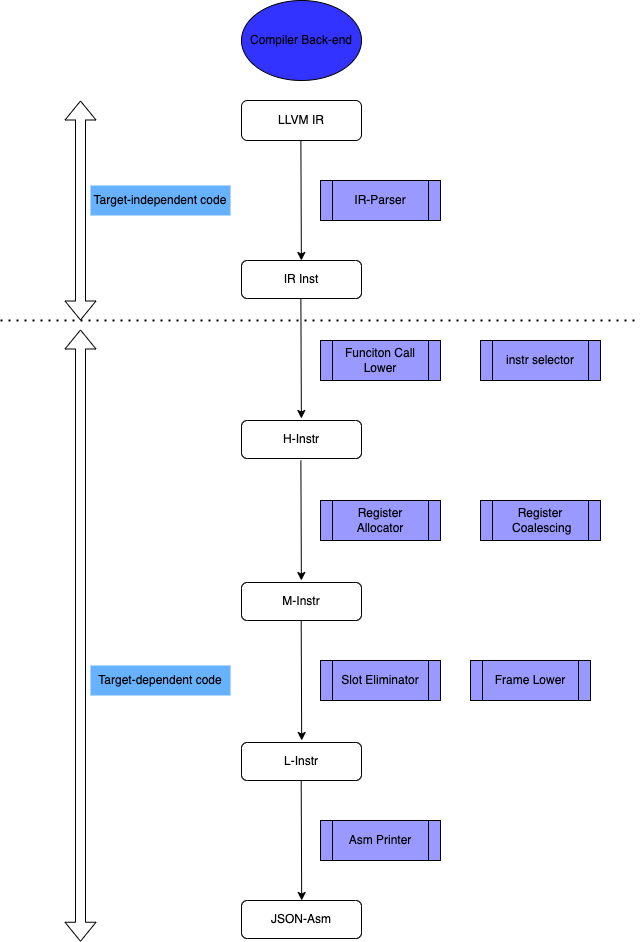
\includegraphics[width=0.6\textwidth]{ola-lang-backend.jpg}
    \caption{ola-lang backend pipeline}
    \label{fig:ola-lang-backend}
\end{figure}

An example ola-lang ola assembly code for computing sqrt of type u32 with prophet version is as follows:
\begin{lstlisting}[language={}]
{
  "program": "u32_sqrt:\n.LBL3_0:\n  mov r3 r1\n  mov r1 r3\n.PROPHET3_0:\n  mov r0 psp\n  mload r0 [r0,0]\n  range r0\n  mul r2 r0 r0\n  assert r2 r3\n  ret\nmain:\n.LBL4_0:\n  add r8 r8 4\n  mstore [r8,-2] r8\n  mov r1 4\n  call sqrt_test\n  add r8 r8 -4\n  end\nsqrt_test:\n.LBL5_0:\n  add r8 r8 6\n  mstore [r8,-2] r8\n  mov r0 r1\n  mstore [r8,-3] r0\n  mload r1 [r8,-3]\n  call u32_sqrt\n  mstore [r8,-4] r0\n  mload r0 [r8,-4]\n  add r8 r8 -6\n  ret\n",
  "prophets": [
    {
      "label": ".PROPHET3_0",
      "code": "%{\n    entry() {\n        cid.y = sqrt(cid.x);\n    }\n%}",
      "inputs": [
        "cid.x"
      ],
      "outputs": [
        "cid.y"
      ]
    }
  ]
}
\end{lstlisting}

An example ola-lang ola assembly code for computing sqrt of type u32 with instructions version is as follows:
\begin{lstlisting}[language={}]
{
  "program": "main:\n.LBL5_0:\n  add r8 r8 4\n  mstore [r8,-2] r8\n  mov r1 4\n  call sqrt_test\n  add r8 r8 -4\n  end\nsqrt_test:\n.LBL6_0:\n  add r8 r8 19\n  mstore [r8,-16] r1\n  mov r1 0\n  mstore [r8,-17] r1\n  mload r1 [r8,-16]\n  gte r2 r1 3\n  neq r0 r1 3\n  and r2 r2 r0\n  cjmp r2 .LBL6_1\n  jmp .LBL6_2\n.LBL6_1:\n  mload r0 [r8,-16]\n  mstore [r8,-17] r0\n  mload r0 [r8,-16]\n  mstore [r8,-12] r0\n  mload r0 [r8,-12]\n  mov r1 r0\n  mov r2 2\n.PROPHET6_0:\n  mov r0 psp\n  mload r0 [r0,0]\n  mstore [r8,-11] r0\n  mload r0 [r8,-11]\n  range r0\n  mov r0 2\n  mload r1 [r8,-11]\n  add r4 r1 1\n  not r7 r4\n  add r7 r7 1\n  add r5 r0 r7\n  range r5\n  mload r0 [r8,-12]\n  mov r1 r0\n  mov r2 2\n.PROPHET6_1:\n  mov r0 psp\n  mload r0 [r0,0]\n  range r0\n  mul r1 r0 2\n  mstore [r8,-15] r1\n  mload r1 [r8,-15]\n  mload r2 [r8,-11]\n  add r1 r1 r2\n  mstore [r8,-14] r1\n  mload r1 [r8,-14]\n  mload r2 [r8,-12]\n  assert r1 r2\n  add r0 r0 1\n  mstore [r8,-13] r0\n  mload r0 [r8,-13]\n  range r0\n  mload r0 [r8,-13]\n  mstore [r8,-18] r0\n  mov r0 0\n  mstore [r8,-19] r0\n  jmp .LBL6_4\n.LBL6_2:\n  mload r0 [r8,-16]\n  neq r0 r0 0\n  cjmp r0 .LBL6_10\n  jmp .LBL6_11\n.LBL6_3:\n  mload r0 [r8,-17]\n  add r8 r8 -19\n  ret\n.LBL6_4:\n  mload r0 [r8,-19]\n  mov r1 100\n  gte r1 r1 r0\n  neq r3 r0 100\n  and r1 r1 r3\n  cjmp r1 .LBL6_5\n  jmp .LBL6_7\n.LBL6_5:\n  mload r0 [r8,-18]\n  mload r1 [r8,-17]\n  gte r0 r0 r1\n  cjmp r0 .LBL6_8\n  jmp .LBL6_9\n.LBL6_6:\n  mload r1 [r8,-19]\n  add r0 r1 1\n  mstore [r8,-19] r0\n  jmp .LBL6_4\n.LBL6_7:\n  jmp .LBL6_3\n.LBL6_8:\n  jmp .LBL6_7\n.LBL6_9:\n  mload r0 [r8,-18]\n  mstore [r8,-17] r0\n  mload r0 [r8,-16]\n  mstore [r8,-3] r0\n  mload r0 [r8,-18]\n  mstore [r8,-2] r0\n  mload r0 [r8,-3]\n  mov r1 r0\n  mload r0 [r8,-2]\n  mov r2 r0\n.PROPHET6_2:\n  mov r0 psp\n  mload r0 [r0,0]\n  mstore [r8,-1] r0\n  mload r0 [r8,-1]\n  range r0\n  mload r0 [r8,-1]\n  add r4 r0 1\n  not r7 r4\n  add r7 r7 1\n  mload r0 [r8,-2]\n  add r5 r0 r7\n  range r5\n  mload r0 [r8,-3]\n  mov r1 r0\n  mload r0 [r8,-2]\n  mov r2 r0\n.PROPHET6_3:\n  mov r0 psp\n  mload r0 [r0,0]\n  range r0\n  mload r1 [r8,-2]\n  mul r1 r0 r1\n  mstore [r8,-10] r1\n  mload r1 [r8,-10]\n  mload r2 [r8,-1]\n  add r1 r1 r2\n  mstore [r8,-9] r1\n  mload r1 [r8,-9]\n  mload r2 [r8,-3]\n  assert r1 r2\n  mload r1 [r8,-18]\n  add r0 r0 r1\n  mstore [r8,-5] r0\n  mload r0 [r8,-5]\n  range r0\n  mload r0 [r8,-5]\n  mov r1 r0\n  mov r2 2\n.PROPHET6_4:\n  mov r0 psp\n  mload r0 [r0,0]\n  mov r4 r0\n  range r4\n  mov r0 2\n  add r1 r4 1\n  mstore [r8,-8] r1\n  mload r1 [r8,-8]\n  not r7 r1\n  add r7 r7 1\n  add r0 r0 r7\n  mstore [r8,-7] r0\n  mload r0 [r8,-7]\n  range r0\n  mload r0 [r8,-5]\n  mov r1 r0\n  mov r2 2\n.PROPHET6_5:\n  mov r0 psp\n  mload r0 [r0,0]\n  range r0\n  mul r1 r0 2\n  mstore [r8,-6] r1\n  mload r1 [r8,-6]\n  add r1 r1 r4\n  mstore [r8,-4] r1\n  mload r1 [r8,-5]\n  mload r2 [r8,-4]\n  assert r2 r1\n  mstore [r8,-18] r0\n  jmp .LBL6_6\n.LBL6_10:\n  mov r0 1\n  mstore [r8,-17] r0\n  jmp .LBL6_11\n.LBL6_11:\n  jmp .LBL6_3\n",
  "prophets": [
    {
      "label": ".PROPHET6_0",
      "code": "%{\n    function mod(felt x, felt y) -> felt {\n        return x % y;\n    }\n    entry() {\n        cid.r = mod(cid.x, cid.y);\n    }\n%}",
      "inputs": [
        "cid.x",
        "cid.y"
      ],
      "outputs": [
        "cid.r"
      ]
    },
    {
      "label": ".PROPHET6_1",
      "code": "%{\n    function div(felt x, felt y) -> felt {\n        return x / y;\n    }\n    entry() {\n        cid.q = div(cid.x, cid.y);\n    }\n%}",
      "inputs": [
        "cid.x",
        "cid.y"
      ],
      "outputs": [
        "cid.q"
      ]
    },
    {
      "label": ".PROPHET6_2",
      "code": "%{\n    function mod(felt x, felt y) -> felt {\n        return x % y;\n    }\n    entry() {\n        cid.r = mod(cid.x, cid.y);\n    }\n%}",
      "inputs": [
        "cid.x",
        "cid.y"
      ],
      "outputs": [
        "cid.r"
      ]
    },
    {
      "label": ".PROPHET6_3",
      "code": "%{\n    function div(felt x, felt y) -> felt {\n        return x / y;\n    }\n    entry() {\n        cid.q = div(cid.x, cid.y);\n    }\n%}",
      "inputs": [
        "cid.x",
        "cid.y"
      ],
      "outputs": [
        "cid.q"
      ]
    },
    {
      "label": ".PROPHET6_4",
      "code": "%{\n    function mod(felt x, felt y) -> felt {\n        return x % y;\n    }\n    entry() {\n        cid.r = mod(cid.x, cid.y);\n    }\n%}",
      "inputs": [
        "cid.x",
        "cid.y"
      ],
      "outputs": [
        "cid.r"
      ]
    },
    {
      "label": ".PROPHET6_5",
      "code": "%{\n    function div(felt x, felt y) -> felt {\n        return x / y;\n    }\n    entry() {\n        cid.q = div(cid.x, cid.y);\n    }\n%}",
      "inputs": [
        "cid.x",
        "cid.y"
      ],
      "outputs": [
        "cid.q"
      ]
    }
  ]
}
\end{lstlisting}

The backend data structure contains mainly lists,insts and mcinsts. The ABI then contains Function call specification and Mapping Relationships to Virtual Memory.

The backend codegen pipeline process:
\begin{itemize}
    \item IR parsing

    \item Function call lowering

    \item Instruction selection

    \item Register Allocation

    \item Slot elimination

    \item Stack frame handling

    \item Assembly printing
\end{itemize}